\chapter{Introduction}\label{chapter_introduction}
\lettrine{R}{eal-time embedded systems} are prevalent in many safety-critical domains, e.g., automotive, avionics, industrial automation, etc., and the correct functionality of the systems depend both on the correctness of the computations and their timing~\cite{Lee2011IntroductionApproach}\cite{WangJiacun2017RES}, e.g., the braking in vehicles, besides applying the appropriate force on the wheel, the time taken to slow (or halt) the vehicle is vital, otherwise accidents can occur if violated. Moreover, safety-critical software should be mapped to hardware efficiently to conserve critical resources such power and energy, which are scarce in embedded systems. So, it should be analyzed rigorously in order to assure functional and timing correctness and should also be power and energy efficient to guarantee extensibility of the software.

Safety-critical software have become complex, e.g., hundreds of end-to-end functions in modern cars, hybrid and autonomous vehicles, etc., so has triggered for more powerful computing architectures such as distributed computing, e.g., executing the braking software over multiple computing units. Since distributed software are normally exposed to a greater degree of permanent and transient, the reliability of safety-critical software should be assured in order to maximize the dependability of the distributed system. In this regard, fault tolerance via redundancy of software and hardware components is the most common approach to increase reliability. However, it incurs additional computation, and consumes more power and energy. Therefore, besides the timing, the reliability of safety-critical software should be assured to maximize the dependability of the system while minimizing power consumption of the distributed software.

In this thesis, we propose formal methods to specify and analyze requirements and software design of safety-critical systems. Formal methods are mathematical techniques and tools which enable unambiguous specification and modeling, and rigorous analysis of systems, e.g., model checking, satisfiability-modulo theories (SMT), etc~\cite{o2017concise}. Moreover, we propose optimization techniques to minimize the power consumption of a distributed safety-critical software. The techniques can be exact or heuristic, respectively, they deliver optimal and near-optimal solutions.

In safety-critical development, requirements specifications should be precise, unambiguous, consistent, etc. In fact, according standards, e.g., ISO 26262, the requirements are expected to be specified in semi-formal or formal languages. Natural language is the de facto method to specify requirements of embedded system including safety-critical systems. Although requirements expressed in natural language are intuitive and expressive, natural language is inherently ambiguous, consequently the specifications are sometimes ambiguous, incomprehensible, inconsistent, etc~\cite{ieereqspecstandard}. Template-based specification and controlled natural language are the two most commonly used methods to improve requirements specifications. The template-based specification methods, e.g., requirements boilerplates~\cite{Hull2011RequirementsEngineering}, etc.,  lack meta-model for extensible and the template selection is usually cumbersome. Controlled natural languages, e.g., Attempto~\cite{attempto96}\cite{Fuchs2008AttemptoRepresentation}, etc., mimic the intuitiveness of natural language and have formal semantics, however, lack support for embedded systems, hence are less effective. 

The specifications are employed in subsequent system development including software design to verify the latter for correct functionality. The software design is usually modeled, simulated and analyzed before implementation. In this regard, Simulink is one of the most widely used development environment for multi-domain, multi-rate, discrete and continuous safety-critical systems in industry~\cite{JamesB.Dabney2003MasteringSimulink}. For this main reason, there is increasing interest in formal analysis of Simulink models~\cite{Manamcheri2011AModels}\cite{Sims2007ExperienceReport}. Simulink Design Verifier, which is based on the Prover model-checker, is the de facto tool in the Simulink environment to formally verify Simulink design models. However, it has limited functionality, e.g., it supports only discrete models, has issues with scalability, and lacks verification of timed properties. 

The software design is mapped to hardware, which should take into consideration effectiveness and efficiency. The software should be effectively mapped to the execution platform, that is satisfying such as the timing and reliability constraints. Furthermore, it should be efficient such as minimizing power consumption to ensure extensibility of the software for future growth. The software-to-hardware allocation is NP-hard, as a result, exact methods are usually used for relatively small problems and heuristics for large and complex problems.

Our research is evaluated on industrial automotive use cases and realistic benchmark. The requirements specification language ReSA and the analysis of Simulink models are evaluated on the adjustable speed-limiter (ASL) and brake-by-wire (BBW) systems provided by Volvo Group Trucks Technology (VGTT). ASL is a speed limitation automotive function which controls the vehicle speed of Volvo trucks from speeding up and is useful in roads where speed-limitation signs are in place. The ASL use case consists of around 300 functional and extra-functional requirements, architectural models in EAST-ADL, and Simulink models. The integrated software allocation is evaluated on the engine management system benchmark provided by Bosch~\cite{}, which consist of an AUTOSAR architecture with the timing specifications, activation mechanisms of schedulable objects employed to model the execution behavior of the system.

\section{Research Contributions Overview}
In this subsection, we give overview of the thesis contributions, and later in Section x, the contributions are further discussed in detail.
\begin{itemize}
\item \textbf{Formal Analysis of natural language requirements:}  we propose a fairly expressive, flexible yet structured and domain-specific constrained natural language, called \textit{ReSA}~\cite{resatool}\cite{Mahmud2015ReSA:Systems}. The language has semantics in Boolean and description logic to support for shallow and rigorous analysis, respectively. The Boolean specifications are checked for consistency using the satisfiability-modulo theory via the Z3 SMT solver. Whereas, the description logic is used to encode the specification as ontology, where we check consistency of the specifications at the lexical level using Reasoner (Inference engine) such Hermit. The ReSA tool, which consists of an editor and implements consistency-checking functionality, is integrated seamlessly into EATOP, which is an open source EAST-ADL IDE, to complement the requirements modeling. 

\item \textbf{Scalable analysis of Simulink models:} we propose a pattern-based, execution-order preserving automatic transformation of atomic and composite Simulink blocks into stochastic timed automata that can be formally analyzed using UPPAAL Statistical Model Checker \cite{Bulychev2012UPPAAL-SMC:Automata}. Our method is scalable, and has been validated on industrial use cases \cite{Filipovikj2016SimulinkSystems}. The statistical model checker analyzes a state-transition system by conducting statistical analysis on the collected traces of the system executions, effectively mitigating the state-space explosion of (exact) model checking \cite{Legay2010StatisticalOverview}. 

\item \textbf{Efficient Power consumption ILP and metaheuristics:} we propose an integer-linear programming (ILP) model to the allocation of distributed software on the network of heterogeneous computing units, which have different processor speed, failure rate and power consumption specifications. The ILP implemented in JAVA using the ILOG CPLEX interface, and subsequently solved the CPLEX solver.
\item \textbf{Validation on industrial use cases: } 
Our contributions such as its the ReSA language as well as the proposed formal analysis of Simulink model is validated on industrial use cases, which are provided
\end{itemize}
% \begin{figure}
% 	\centering
% 	\ifpdf
% 	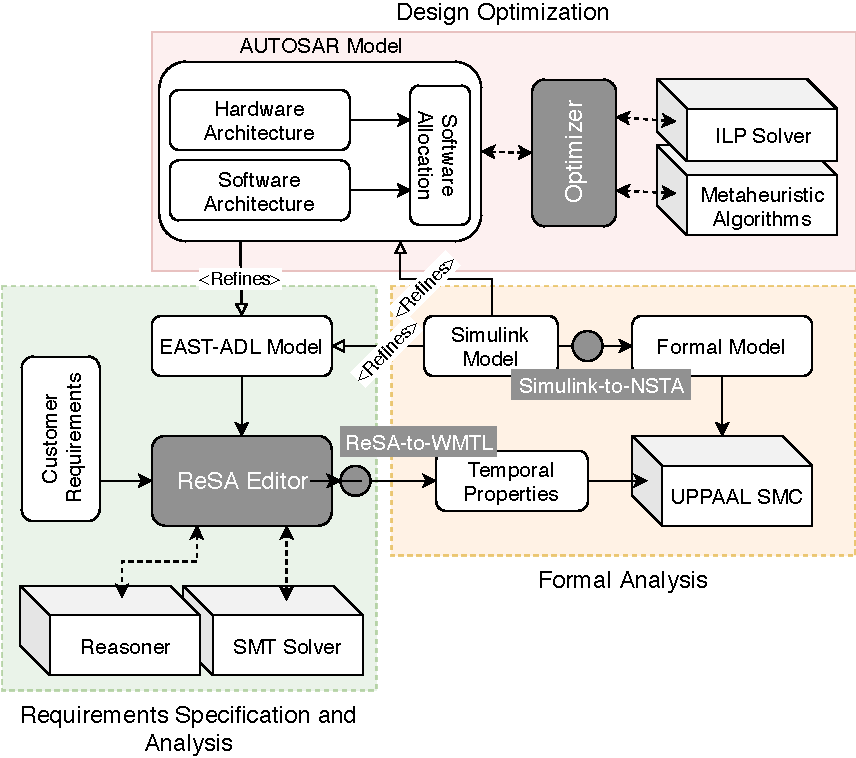
\includegraphics[width=\linewidth]{images/softdevflow}
% 	\else
% 	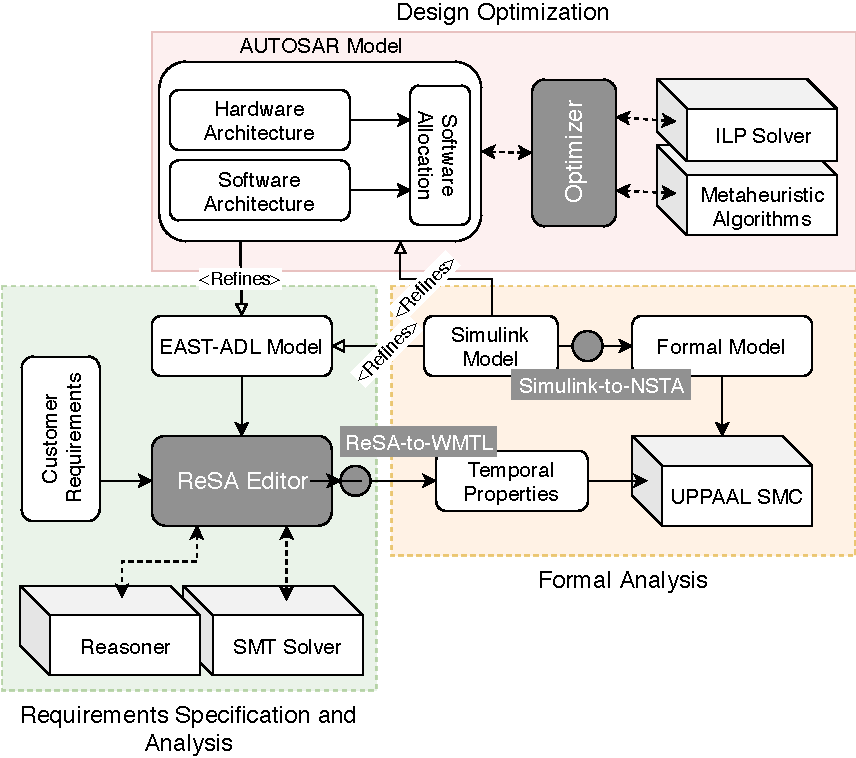
\includegraphics[width=1.0\linewidth]{images/softdevflow.eps}
% 	\fi
% 	\caption{Thesis Contributions Workflow.} 
% \end{figure}

\section{Thesis Outline Overview}
The thesis is divided into two parts. The first part is a summary of our research. It is organized as follows: in Chapter 2, we give the background information on description logic, Boolean satisfiability problem, Simulink, stochastic timed automata, and meta-heuristic optimization. In Chapter 3, we explain the research problem and outline the research goals. The thesis contributions are discussed in Chapter 4, followed by the related work in Chapter 5. In Chapter 3, we describe the research method applied to conduct the research. Finally, in Chapter 7, we conclude the thesis and outline possible directions for future work.
